\vspace{-.5cm}
\section{Tool Demonstration}
\label{sec:demo}
\vspace{-.3cm}
In this section, we discuss the main steps of the process that need to be
followed for synthesizing the EARS-CTRL specification into a controller and
validating if the controller behaves as expected.
\vspace{-.3cm}
\subsection{Glossary building and terms definition}
\vspace{-.2cm}
The first step towards writing the controller specifications in natural
language using \textsf{EARS-CTRL} is to define the glossary terms. 
The user is provided with an editor
(figure~\ref{fig:glossary_def}) to define glossary terms for:
1) components that interface with the controller; 2) sensors and actuators those
components make available to the controller and 3) invariant relations
that should hold between the sensor and actuator signals and aliases to
formulas involving sensors or actuators for ease of writing.\levi{check for new
version of the glossary for the QC}
\vspace{-.2cm}
\begin{figure*}[!h]
\centering
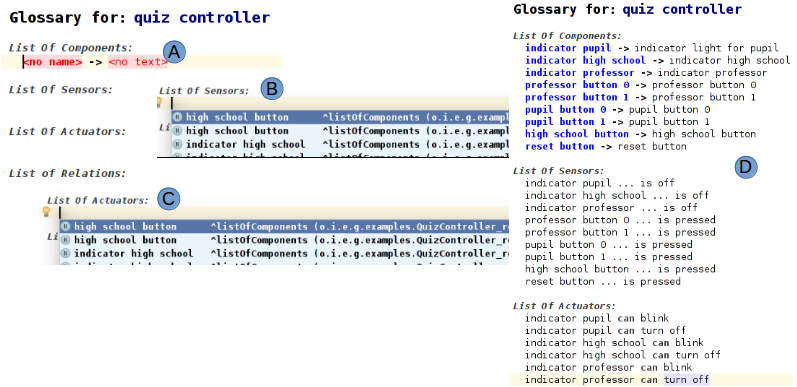
\includegraphics[width=1\textwidth]{./images/QC_Glossary_Def.png}
\caption{Step-by-step glossary building for a Quiz Controller: (\emph{A})
components definition, (\emph{B}) sensors definition, (\emph{C}) actuators
definition and (\emph{D}) completed QC glossary}
\label{fig:glossary_def}
\end{figure*}
\vspace{-.2cm}
\subsection{Building \textsf{EARS-CTRL} requirements for the Quiz Controller}
\vspace{-.2cm}
The user is provided with an editor built in MPS \cite{mps} to specify the
controller behavior. The user can input the requirements simply by filling in
the instance of the EARS template with placeholders in the editor\levi{I don't
think this sentence is necessary}.
Figure~\ref{fig:EARS_req} provides step-by-step guidance to write the EARS
requirements. In the projectional editor the user is provided with the option
(i.e., using \emph{CTRL+Space} keys of the keyboard) to instantiate the
EARS-based template with placeholders (\emph{Step A}). After obtaining an
instance of the EARS template, the user fills in the placeholders with
information coming from the glossary definitions (\emph{Step B}). \emph{Step C}
of the figure~\ref{fig:EARS_req} depicts a complete Quiz Controller specification.
\begin{figure*}[!h]
\centering
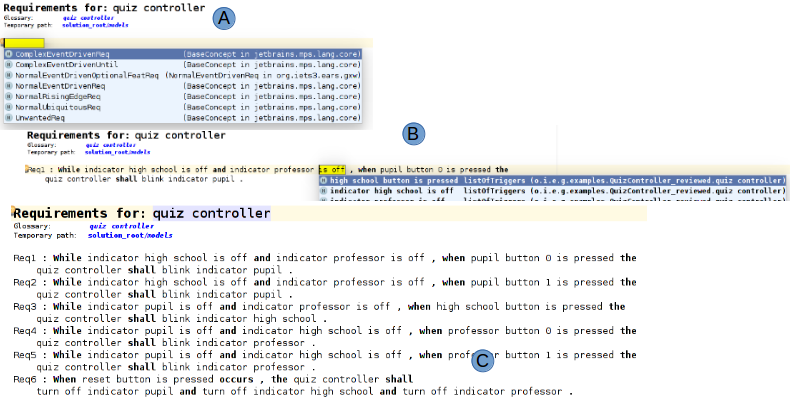
\includegraphics[width=1.2\textwidth]{./images/Req_Spec_Steps.png}
\caption{Step-by-step \textsf{EARS-CTRL} for controller requirements: (\emph{A})
Empty instance of EARS template with placeholders, (\emph{B}) Filling instance of an EARS
template with information and (\emph{C}) Completed EARS Specification }
\label{fig:EARS_req}
\end{figure*}
\vspace{-.2cm}
\subsection{Synthesizing \textsf{EARS-CTRL} requirements}
\vspace{-.2cm}
Once the requirements for controller are completely specified, the user can
attempt to synthesize the controller. For that, the user can apply the
\emph{Transform} intention (i.e., by using the \emph{Alt+Enter} keys) on the root of the specification (as
shown in \emph{part A} of figure~\ref{fig:Spec_transform}). The generated outputs after applying the
intention are comprised of: 1) the \emph{Controller Holder}, Data Flow
Diagram (DFD) with blocks and wires (\emph{part B} of
figure~\ref{fig:Spec_transform}); and 2) the \emph{Gate Descriptors}, pseudo
code representing the behavior of each of the blocks used by the synthesized controller (\emph{part C} of
figure~\ref{fig:Spec_transform}).
%\vspace{-.7cm}
\begin{figure*}[!h]
\centering
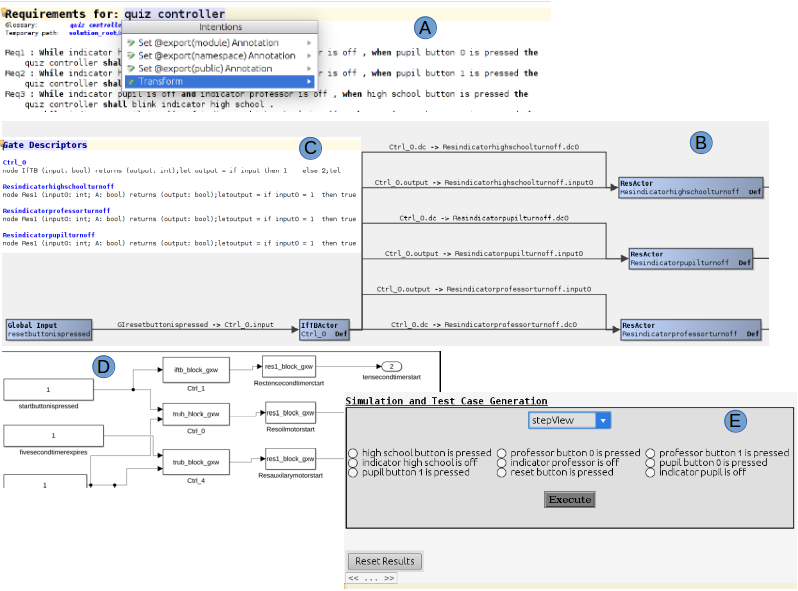
\includegraphics[width=1\textwidth]{./images/Transform.png}
\caption{Controller generation steps: (\emph{A}) applying intention \emph{Alt+Enter},
(\emph{B}) synchronized DFD of the controller (an excerpt)
and (\emph{C}) pseudo code representing the behavior of the blocks (an excerpt)}
\label{fig:Spec_transform}
\end{figure*}
\vspace{-.5cm}
\subsection{Simulation and Test Cases for Validation of Controller Behavior}
\vspace{-.2cm}
Validation of the generated controller to check if it behaves as expected can be
performed using following techniques: 1) simulating the behavior of the
controller step-by-step; and 2) automatically generating the test cases.
The resulting traces from simulation or test generation are analyzed in order to
check if the controller behaves as expected.
%\vspace{-.5cm}
\subsubsection{Simulation}
\vspace{-.2cm}
In order to perform simulation of the generated controller, the user
starts by applying the \emph{GenerateSimulinkModel} intention on the root of the
\emph{Controller Holder} (i.e., \emph{Step A}  in
figure~\ref{fig:SimulationSteps}) to generate the Simulink counterpart of the
controller\levi{this could be done in only one step together with the SDF
controller}.
After having the Simulink model generated, the user can apply the intention
\emph{AddOutputChecker} (i.e., \emph{Step B and C} in figure
~\ref{fig:SimulationSteps}) to start simulating the controller behavior by
providing manual input. For simulation purpose, the user gets the
\textsf{EARS-CTRL} panel that allows the user to simulate the controller by
providing a sequence of inputs manually.\levi{is this sentence necessary?}
Outputs are incrementally added to the panel as new inputs are provided by the
requirements engineer (i.e., \emph{Step D} in figure~\ref{fig:SimulationSteps}).
A \textsf{“Reset Results”} button enables the user to reset the controller to
its initial state. 
\begin{figure*}[!h]
\centering
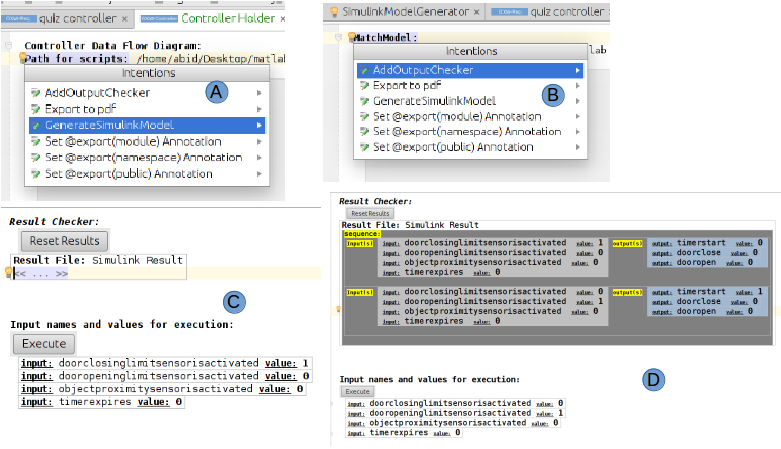
\includegraphics[width=1\textwidth]{./images/Simulation_Steps.png}
\caption{Simulation steps for validation: (\emph{A}) applying
GenerateSimulinkModel Intention, (\emph{B}) applying intention
\textsf{AddOutputChecker} , (\emph{C}) generated empty
\textsf{EARS-CTRL} panel and (\emph{D}) manually simulating the controller}
\label{fig:SimulationSteps}
\end{figure*}
\vspace{-.3cm}
\subsubsection{Automatic Test Cases Generation} 
\vspace{-.5cm}
The user can automatically generate test cases
(figure~\ref{fig:TestCaseGeneration}) by setting in the testing parameters.
For the test case generation, the user inputs the
parameters in the \textsf{EARS-CTRL} panel.
The parameters required for test case generation are as follows, 1) \textsf{Test
Sequence Length(integer value)}, 2) \textsf{Allow parallel inputs(true/false)} and 3) \textsf{Allow repeated inputs (true/false)}.